
\documentclass[12pt]{article}

%	页面设置
\usepackage{geometry}
\geometry{left=2.5cm, right=2.5cm, top=2.5cm, bottom=2.5cm}
\usepackage{graphicx}
\usepackage{ctex}
\usepackage{fontspec}
\usepackage{setspace}
\usepackage{array,longtable,subcaption,multirow,float,calc,tcolorbox}
\usepackage{siunitx}
\usepackage[version=4]{mhchem}
\usepackage{inconsolata}
\usepackage[strict]{changepage}
\usepackage{listings}
\usepackage{xcolor} % for setting colors

% Define your colors here
\definecolor{codegray}{gray}{0.9}

% Set up the listings package to format the code
\lstnewenvironment{code}{
    \lstset{
        backgroundcolor=\color{codegray}, % set the background color
        basicstyle=\ttfamily, % set the font style to teletype family
        breaklines=true, % allows line breaking
        numbers=left, % line numbers on the left
        numberstyle=\tiny\color{gray}, % style for the line numbers
        stepnumber=1, % numbering steps
        numbersep=5pt, % how far the line numbers are from the code
        frame=none, % no frame around the code
        framesep=0pt, % space before and after the code (if no frame, not needed)
        rulecolor=\color{black}, % frame color (if no frame, not needed)
        framerule=0pt, % frame thickness (if no frame, not needed)
        fillcolor=\color{codegray}, % background color (if not using the general backgroundcolor)
        tabsize=4, % tab size
        showstringspaces=false, % don't mark spaces in strings
        aboveskip=1pt, % reduces the default spacing above the code block
        belowskip=2pt, % reduces the default spacing below the code block
        % any other code settings can be added here
    }
}{}



%\usepackage{etoolbox}
%\robustify\ref
%\pretocmd{\ref}{\textbf}{}{}

%	字体设置
\setmainfont{Times New Roman}
\setCJKmainfont{SimSun.ttf}
\setCJKsansfont{SimHei.ttf}

%	表格设置
\usepackage{makecell}
\newcommand{\addcell}[2][4]{\makecell{\zihao{#1}\textsf{#2}}}
\usepackage{titlesec}
\usepackage{booktabs}
\usepackage{tabularx}

%	设置图注、表注
\usepackage{caption}
\usepackage{bicaption}
\captionsetup{labelsep=quad, font={small, bf}, skip=2pt}
\DeclareCaptionOption{english}[]{
    \renewcommand\figurename{Fig.}
    \renewcommand\tablename{Table}
}
\captionsetup[bi-second]{english}

%	设置页眉
\usepackage{fancyhdr}
\pagestyle{fancy}
\fancypagestyle{preContent}{
    \fancyhead[L]{\zihao{-5} 物理化学实验}
    \fancyhead[C]{\zihao{-5} 实验三\ \ 液体饱和蒸气压的测定}
    \fancyhead[R]{\zihao{-5} 2100011873\ 王子宸}
}
\pagestyle{preContent}

%	设置首页页眉及取消首页页脚 若不需要首页页眉 请注释掉下列内容
%\fancypagestyle{plain}{
	%\fancyhead[L]{\zihao{-5} 物理化学实验}
	%\fancyhead[C]{\zihao{-5} 实验xx\ \ xxxxx}
	%\fancyhead[R]{\zihao{-5} xxxxxxxxxx\ xxx}
	%\cfoot{}
%}

%	设置标题格式
\titleformat*{\section}{\zihao{4}\sffamily}
\titleformat*{\subsection}{\zihao{-4}\sffamily}
\titleformat*{\subsubsection}{\zihao{-4}\sffamily}
\titlespacing*{\section}{0pt}{10pt}{10pt}
\titlespacing*{\subsection}{0pt}{10pt}{5pt}
\titlespacing*{\subsubsection}{0pt}{10pt}{5pt}

%	设置引用格式(ACS格式规范)
%	注意:请安装JabRef
%	JabRef使用参考:https://blog.csdn.net/weixin_44191286/article/details/85698921
\usepackage[super,round,comma,compress]{natbib}

%	数学公式增强
\usepackage{amsmath}
\usepackage{amssymb}

\newcolumntype{M}[1]{>{\centering\arraybackslash}m{#1}}
%	设置封面
\begin{document}
    % 标题页

\begin{titlepage}
% 页眉
\thispagestyle{plain}
% 校徽图片
\begin{figure}[h]
    \centering
    \includegraphics{pku.png}
\end{figure}
\vspace{24pt}
% 标题
\centerline{\zihao{-0} \textsf{物理化学实验报告}}
\vspace{40pt} % 空行
\begin{center}
    \begin{tabular}{cc}
        % 题目
        
        \addcell[2]{题目:\ } & \addcell[2]{紫外可见吸收光谱仪的搭建 与} \\
        \cline{2-2}\\
        & \addcell[2]{量子一维势阱方程的检验}\\
        \cline{2-2}
        
    \end{tabular}
\end{center}
\vspace{20pt} % 空行
\begin{center}
    \doublespacing
    \begin{tabular}{cp{5cm}}
        % 姓名
        \addcell{姓\phantom{空格}名:\ } & \addcell{王子宸} \\
        \cline{2-2}
        % 学号
        \addcell{学\phantom{空格}号:\ } & \addcell{2100011873}\\
        \cline{2-2}
        % 组别
        \addcell{组\phantom{空格}别:\ } & \addcell{周四19组8号} \\
        \cline{2-2}
        % 实验日期
        \multirow{2}{*}{\addcell{实验日期:\ }} & \addcell{\zhdate{2023/10/26}}\\
        \cline{2-2}
        & \addcell{\zhdate{2023/11/2}}\\
        \cline{2-2}
        % 室温
        \addcell{室\phantom{空格}温:\ } & \addcell{20.6\si{^\circ C}\ \ 21.7\si{^{\circ}C}}\\
        \cline{2-2}
        % 大气压强
        \addcell{大气压强:\ } & \addcell{100.95\si{kPa}\quad99.90\si{kPa}}\\
        \cline{2-2}
    \end{tabular}
    \begin{tabular*}{\textwidth}{c}
    \\
    \\
        \hline % 分割线
    \end{tabular*}
\end{center}
% 摘要
\textsf{摘\ \ 要}\ \ 本实验利用实验室提供的部件搭建了紫外可见吸收光谱仪,利用氘灯对光谱仪进行了调试和标定;用光谱仪测定了同一物质不同浓度溶液的吸收光谱,拟合工作曲线,验证了 Lambert-Beer 定律,并对比了使用氘灯光源和卤钨灯光源的差异;测量了多个共轭分子的吸收光谱,计算了各分子的摩尔吸光系数 $\varepsilon $;分别用一维势阱模型和 Gaussian 程序对各分子进行了模拟计算,比较了计算结果与实验结果的差别。
\\
\\
% 关键字
\textsf{关键词}\ \ 物理化学实验;紫外-可见吸收光谱仪;一维势阱模型;花菁染料;TDDFT
\end{titlepage}

\section{引言}

\subsection{实验目的与原理}

\begin{figure}[H]
    \centering
    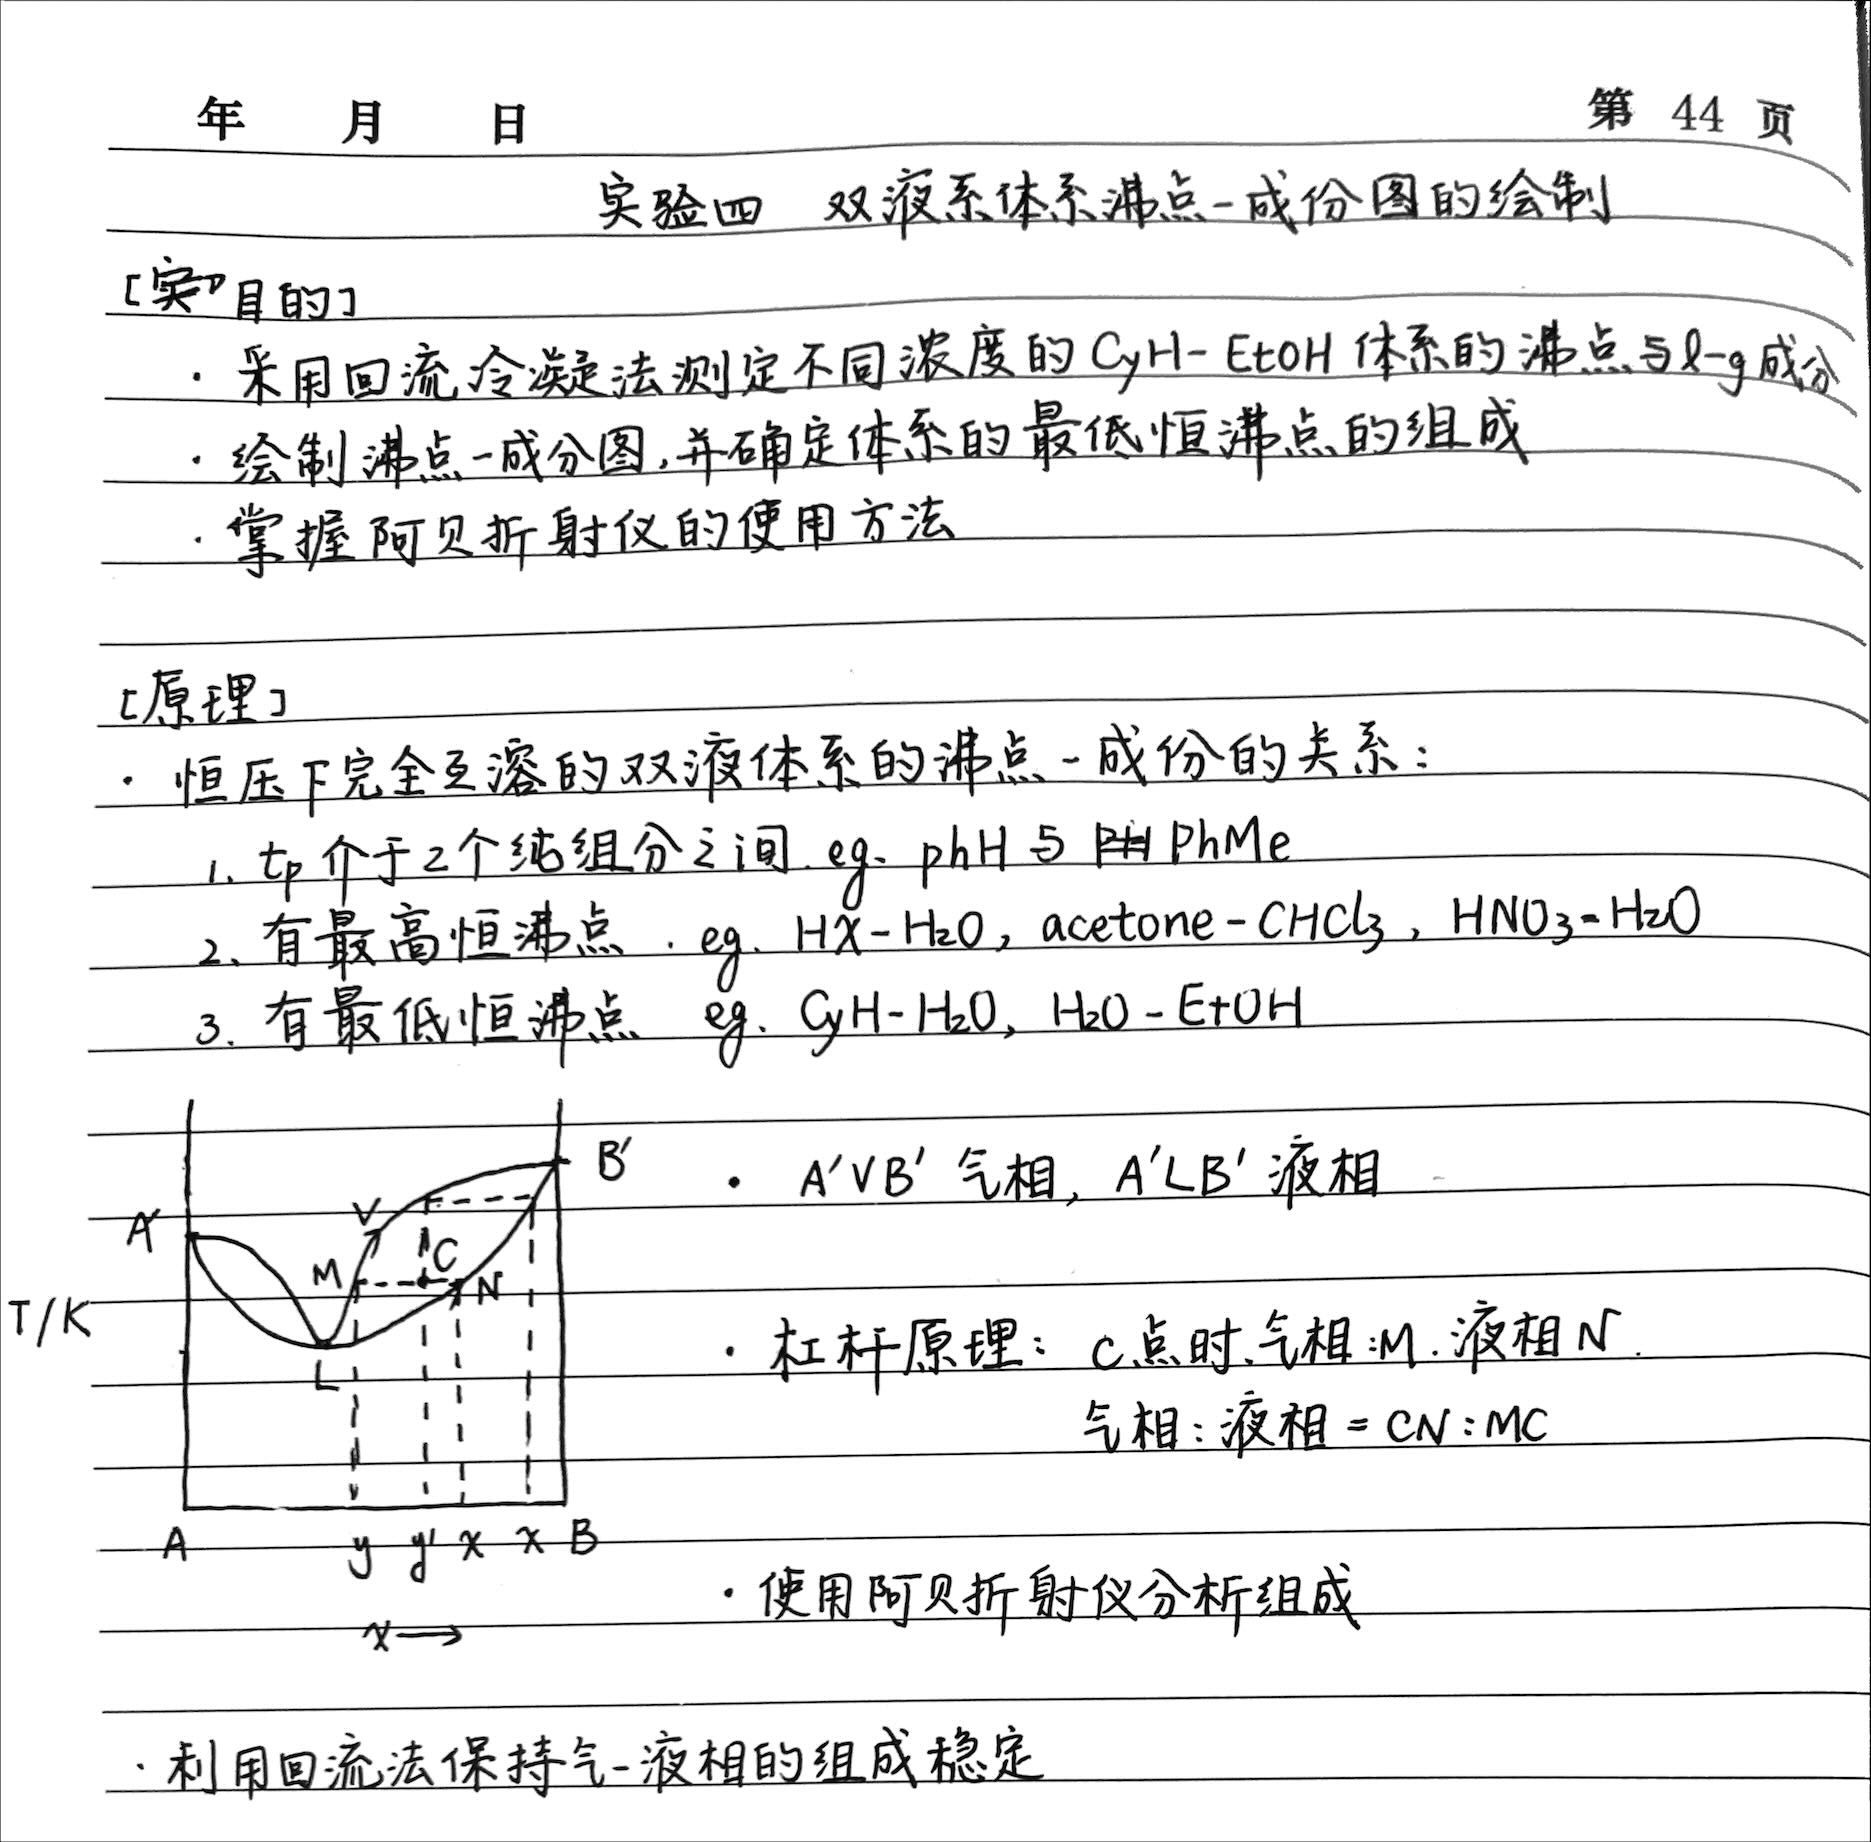
\includegraphics[width=.8\textwidth]{figures/0-1.jpg}
    \bicaption{预习报告:实验的目的与原理(1)}{Preview Report: Purpose and Principle of the Experiment 1}
\end{figure}

\begin{figure}[H]
    \centering
    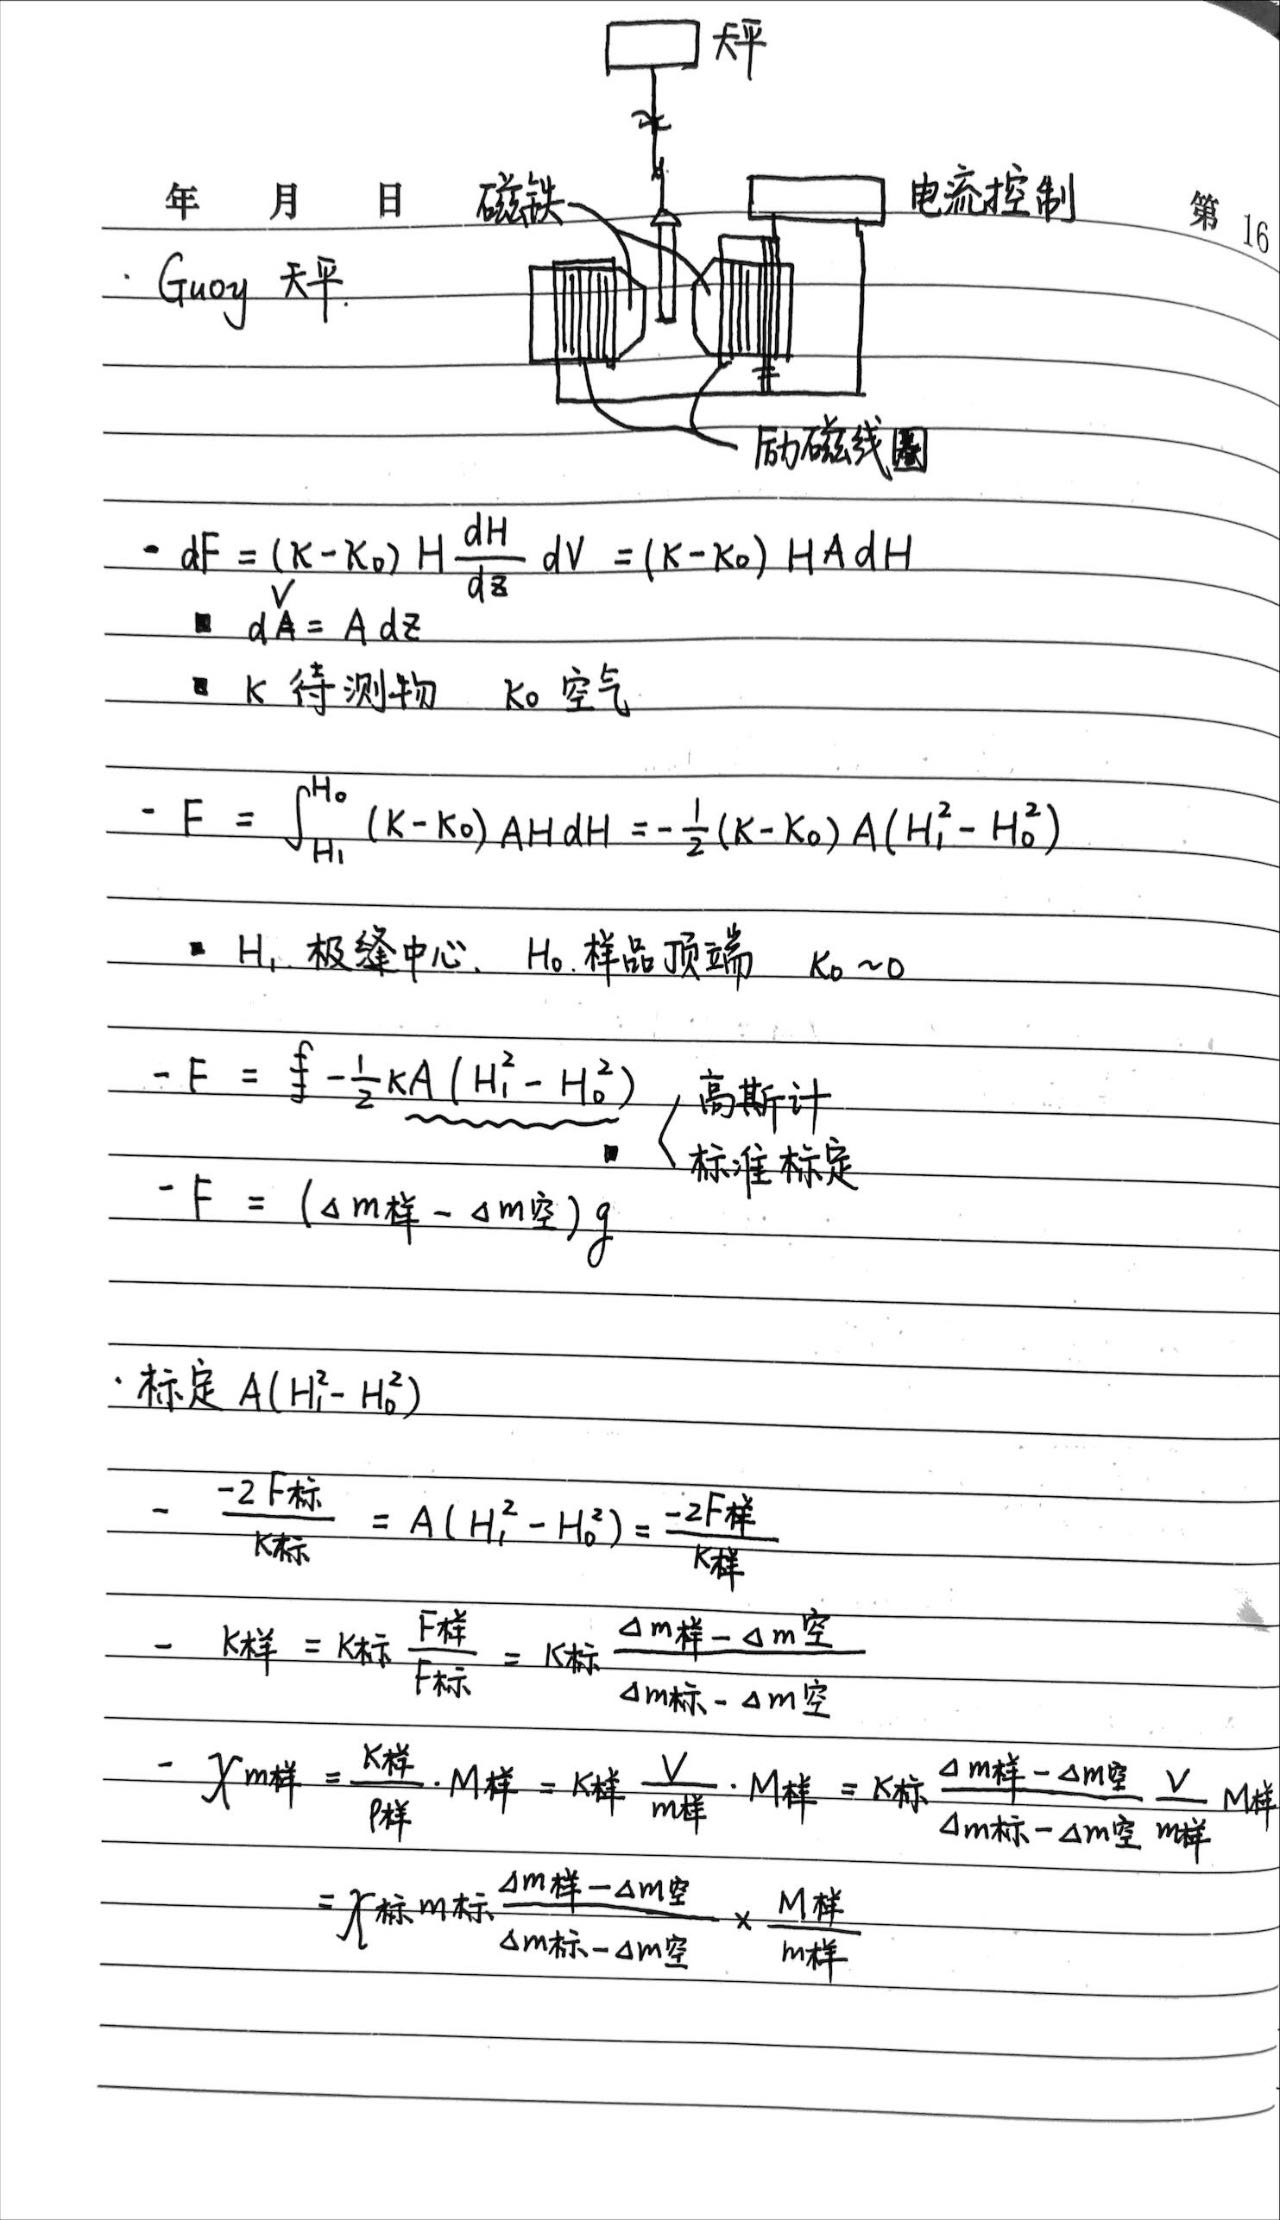
\includegraphics[width=.8\textwidth]{figures/0-2.jpg}
    \bicaption{预习报告:实验的目的与原理(2)}{Preview Report: Purpose and Principle of the Experiment 2}
\end{figure}




\section{实验内容\cite{pcl2002}}

\subsection{仪器与药品}

蔗糖 (AR), 盐酸 $(\mathrm{AR}, 2.96 \mathrm{~mol} / \mathrm{L}, 3.95 \mathrm{~mol} / \mathrm{L}, 5.85 \mathrm{~mol} / \mathrm{L})$ 。

旋光仪, 秒表, 恒温旋光管, 烧杯 $(500 \mathrm{~mL})$, 移液管 $(25 \mathrm{~mL}$ 若干), 磨口雉形瓶 $(100 \mathrm{~mL} \times 5)$, 量筒 $(100 \mathrm{~mL})$, 水浴装置, 电子台秤 $(0.01 \mathrm{~g})$ 。

\subsection{实验步骤与条件}

\subsubsection{旋光仪的使用和校零}

接通 WXG-4 目视旋光仪电源, 打开电源开关预热 $10 \mathrm{~min}$, 待完全发出钠黄光。洗净恒温旋光管, 连接好恒温水管路, 将旋光管加满去离子水, 并将管内气泡从加液口排净, 旋光管外壁残液用滤纸擦净、两端玻璃片用擦镜纸擦净, 放入旋光仪镜筒中。调节调焦螺旋,使视场中三分视场分界线最清晰。调节读盘转动手轮, 至三分视场消失, 视野暗度相同, 从读数放大盘中读出度盘的示数, 即为旋光仪零点的旋光度 $\alpha$ 。重复测量旋光仪零点 5 次, 取平均值作为旋光仪的零点。

\subsubsection{配制蔗糖溶液}

用粗天平称取 $30.03 \mathrm{~g}$ 蔗糖, 加入 $150.0 \mathrm{~mL}$ 蒸馏水, 在 $250 \mathrm{~mL}$ 烧杯中搅拌溶解。

\subsubsection{旋光度的测定}

用移液管移取 $25.00 \mathrm{~mL}$ 蔗糖溶液置于干燥的 $100 \mathrm{~mL}$ 雉形瓶中, 置于 $30^{\circ} \mathrm{C}$ 恒温水浴槽中预热。用另一支移液管移取 $25.00 \mathrm{~mL} 6.16 \mathrm{~M}$ 盐酸溶液($1\mathrm{~M}=1\mathrm{~mol\cdot L^{-1}}$), 移入装有蔗糖溶液的雉形瓶中。当酸流入一半时, 打开秒表开始计时。盐酸全部流入后迅速将混合液摇匀。取少量混合液润洗旋光管 $2 \sim 3$ 次, 用混合液装满旋光管。

用滤纸擦净管外壁的溶液, 尽快把旋光管放入旋光仪中, 测量不同时间 $t$ 时溶液的旋光角 $\alpha_t$ 。在反应开始 $15 \mathrm{~min}$ 内, 每半分钟到一分钟记录一次读数, 以后测量的时间间隔适

当加长, 测至旋光角 $\alpha_t$ 由右旋变为左旋, 至少获取 12 组有效数据。测量结束后, 将旋光管中的混合液倒回原雉形瓶中备用。

按照以上步骤, 依次使用 $3.14 \mathrm{~M}$、$4.19 \mathrm{~M}$、$6.16 \mathrm{~M}$ 的盐酸溶液, 进行混合液旋光度的测定。后续 4 组混合液不需倒回原雉形瓶中。()

\subsubsection{$\alpha_{\infty}$ 的测定}

将雉形瓶中保留备用的 $6.16 \mathrm{~M}$ 盐酸溶液与蔗糖溶液的混合液置于恒温水浴槽中预热,取少量混合液润洗旋光管 $2 \sim 3$ 次, 用混合液装满旋光管, 测定混合液的旋光度即为 $\alpha_{\infty}$ 。重复测量 5 次, 取平均值作为 $\alpha_{\infty}$ 的值。



\section{实验结果}

\subsection{溶液表面张力的测定}

\subsubsection{最大气泡压力法}

由于本人所使用的U型压力计,由于固定的原因,左右侧读数零点并无法保证严格的一致。因此,在每次测定前,均记录U型压力计左右侧的零点,记为$h_{0}$,记录一次;然后读取左右侧各自读取3组最大气泡压力时的示数,为$h_{1}$,取平均得到$\bar{h}_1$;分别计算两边的高度差,再相减得到总的高度差$\Delta h$,得到表 \ref{tab:1}:
\begin{equation}\label{eq:3}
    \Delta h = (h_{1,r} - h_{0,r}) - (h_{1,l} - h_{0, l})
\end{equation}


\begin{table}[htbp]
    \centering
    \bicaption{最大气泡压力法的高度差测量结果}{Measurement Results of Height Difference by Maximum Bubble Pressure Method}
    \begin{adjustwidth}{-2cm}{-2cm}
    \begin{center}
    \begin{tabular}{cccccccccccc}
    \toprule
    $c_{n\ce{BuOH}}$ & \multicolumn{5}{c}{左侧液面高度/\si{cm}} & \multicolumn{5}{c}{右侧液面高度/\si{cm}} & $\Delta h$ \\
     /\si{mol\cdot L^{-1}}& $h_{0,l}$ & $h_{1,l,1}$ & $h_{1,l,2}$ & $h_{1,l,3}$ & $\bar{h}_{1,l}$ & $h_{0,r}$ & $h_{1,r,1}$ & $h_{1,r,2}$ & $h_{1,r,3}$ & $\bar{h}_{1,r}$ & /\si{cm} \\
    \midrule
    0.0000 & 18.90 & 14.50 & 14.52 & 14.49 & 14.50 & 18.90 & 23.13 & 23.12 & 23.12 & 23.12 & 8.62 \\
    0.0218 & 18.90 & 14.85 & 14.86 & 14.87 & 14.86 & 18.90 & 22.83 & 22.84 & 22.85 & 22.84 & 7.98 \\
    0.0547 & 18.85 & 15.24 & 15.23 & 15.23 & 15.23 & 18.92 & 22.42 & 22.44 & 22.45 & 22.44 & 7.13 \\
    0.111 & 18.88 & 15.73 & 15.72 & 15.74 & 15.73 & 18.90 & 22.96 & 22.97 & 22.95 & 22.96 & 7.21 \\
    0.220 & 18.87 & 16.22 & 16.25 & 16.23 & 16.23 & 18.91 & 21.50 & 21.51 & 21.52 & 21.51 & 5.24 \\
    0.329 & 18.89 & 16.55 & 16.60 & 16.57 & 16.57 & 18.92 & 21.16 & 21.15 & 21.13 & 21.15 & 4.54 \\
    0.439 & 18.90 & 16.78 & 16.77 & 16.79 & 16.78 & 18.91 & 20.95 & 20.94 & 20.94 & 20.94 & 4.15 \\
    0.550 & 18.87 & 17.01 & 16.99 & 17.00 & 17.00 & 18.93 & 20.76 & 20.75 & 20.75 & 20.75 & 3.69 \\
    0.740 & 18.87 & 17.18 & 17.20 & 17.20 & 17.19 & 18.92 & 20.52 & 20.53 & 20.53 & 20.53 & 3.28 \\
    \bottomrule
    \end{tabular}
    \end{center}
    \end{adjustwidth}
    \label{tab:1}
\end{table}

以纯水作为标准参比,根据:
\begin{gather*}
    p = p^\ominus +\frac{2\gamma}{r} = p^\ominus +\rho g\Delta h \\
    \gamma \propto \Delta h
\end{gather*}

已知,在恒温\SI{30}{{}^\circ C}时,纯水的表面张力为\SI{71.18}{mN\cdot m^{-1}}\cite{haynes2016crc},因此,正丁醇水溶液的表面张力可以由公式 \eqref{eq:1} 计算。
\begin{equation}\label{eq:1}
    \gamma =\frac{\Delta h}{\Delta h_{\ce{H2O}}}\cdot \gamma_{\ce{H2O}}
\end{equation}

进一步,考虑高度测定中的误差,根据表 \ref{tab:1} 中,对于同一高度多次测量的结果,其最大偏差约为\SI{0.05}{cm},因此,不妨假设单次高度测量的读数误差为(在本实验报告中,为了方便起见,略去误差的单位,其单位与其所对应的物理量保持一致):
\begin{equation*}
    \sigma_h = \frac{0.05}{\sqrt{3}} = 0.029
\end{equation*}

根据 \eqref{eq:3},可以得到高度差的不确定度:
\begin{align*}
    \sigma_{\Delta h} &= \sqrt{3\times\left(\frac{\sigma_{h_{1,r}}}{3}\right)^2 + \left(-\sigma_{h_{0,r}}\right)^2 + \left(\sigma_{h_{0,l}}\right)^2  + 3\times\left(-\frac{\sigma_{h_{1,l}}}{3}\right)^2}\\
    &= \sqrt{\frac{8}{3}} \sigma_h = 0.047
\end{align*}
显然,高度差的不确定度与高度差本身的数值无关。

根据公式 \eqref{eq:1},可知:
\begin{align*}
\frac{\partial \gamma }{\partial \Delta h_{\ce{H2O}} }&=- \frac{\gamma_{\ce{H2O}} \Delta h}{\Delta h_{\ce{H2O}}^{2}} \\
\frac{\partial \gamma }{\partial \Delta h }&=\frac{\gamma_{\ce{H2O}}}{\Delta h_{\ce{H2O}}} \\
\sigma_\gamma &=\sqrt{\left(\frac{\partial \gamma }{\partial \Delta h_{\ce{H2O}} } \sigma_{\Delta h_{\ce{H2O}}}\right)^2+\left(\frac{\partial \gamma }{\partial \Delta h } \sigma_{\Delta h}\right)^2}\\
&= \sqrt{\left(- \frac{\gamma_{\ce{H2O}} \Delta h}{\Delta h_{\ce{H2O}}^{2}}\right)^2 + \left(\frac{\gamma_{\ce{H2O}}}{\Delta h_{\ce{H2O}}} \right)^2}\sigma_{\Delta h} \\
&= \frac{\sigma_{\Delta h}\gamma_{\ce{H2O}}}{\Delta h_{\ce{H2O}}}\sqrt{\frac{ \Delta h^2}{\Delta h_{\ce{H2O}}^{2}} + 1}
\end{align*}

最终,计算得到不同浓度正丁醇溶液的表面张力,如表 \ref{tab:2}。

\begin{table}[H]
    \centering
    \bicaption{最大气泡压力法测得的表面张力}{Surface Tension Measured by Maximum Bubble Pressure Method}
    \begin{tabular}{cccc}
    \toprule
    $c$/\si{mol\cdot L^{-1}} & $\ln \left(c_{n\ce{BuOH}}/\si{mol\cdot L^{-1}}\right)$ & $\Delta h$/\si{cm} & $\gamma$/\si{mN\cdot m^{-1}} \\
    \midrule
        0.0000 & $-$ & 8.62 & 71.18 \\
        0.0218 & -3.826 & 7.98 & 65.90 $\pm$ 0.53 \\
        0.0547 & -2.906 & 7.13 & 58.90 $\pm$ 0.50 \\
        0.111 & -2.198 & 6.21 & 51.28 $\pm$ 0.48 \\
        0.220 & -1.514 & 5.24 & 43.24 $\pm$ 0.45 \\
        0.329 & -1.112 & 4.54 & 37.52 $\pm$ 0.44 \\
        0.439 & -0.823 & 4.15 & 34.30 $\pm$ 0.43 \\
        0.550 & -0.598 & 3.69 & 30.50 $\pm$ 0.42 \\
        0.740 & -0.301 & 3.28 & 27.11 $\pm$ 0.42 \\
    \bottomrule
    \end{tabular}
    \label{tab:2}
\end{table}

\subsubsection{吊片法}

依次使用表面张力仪测量纯水与不同浓度的正丁醇水溶液的表面张力,记录得到表 \ref{tab:3}。由于仪器示数并不稳定,会存在较大范围的波动,因此,最终读数的确定有一定的随机性。

\begin{table}[H]
    \centering
    \bicaption{吊片法测得的表面张力}{Surface Tension Measured by the Wilhelmy Plate Method}
    \begin{tabular}{cccc}
    \toprule
    $c$/\si{mol\cdot L^{-1}} & $\ln \left(c_{n\ce{BuOH}}/\si{mol\cdot L^{-1}}\right)$ &  $\gamma$/\si{mN\cdot m^{-1}} & $T$/\si{{}^{\circ}C} \\
    \midrule
    0.0000 & $-$ & 71.72 & 22.9 \\
    0.0218 & -3.826 & 66.80 & 22.7 \\
    0.0547 & -2.906 & 61.20 & 22.8 \\
    0.111 & -2.198 & 54.56 & 23.1 \\
    0.220 & -1.514 & 48.40 & 22.9 \\
    0.329 & -1.112 & 42.20 & 23.1 \\
    0.439 & -0.823 & 37.90 & 23.1 \\
    0.550 & -0.598 & 34.45 & 23.0 \\
    0.740 & -0.301 & 30.55 & 22.9 \\
    \bottomrule
    \end{tabular}
    \label{tab:3}
\end{table}

\subsection{饱和吸附量与分子吸附面积的计算}

考虑真实界面 $\bar{G}^S=\bar{G}^S\left(T, P, A, n_i^S\right)$ 和理想的参考界面 $\bar{G}^R=\bar{G}^R\left(T, P, n_i^R\right)$,由于是理想界面,因此表面积对 $\bar{G}^R$ 影响,有:

$$
\begin{gathered}
\mathrm{d} \bar{G}^R=\left(\frac{\partial \bar{G}^R}{\partial T}\right) \mathrm{d} T+\left(\frac{\partial \bar{G}^R}{\partial P}\right) \mathrm{d} P+\sum_i\left(\frac{\partial \bar{G}^R}{\partial n_i^R}\right) \mathrm{d} n_i^R \\
\mathrm{~d} \bar{G}^S=\left(\frac{\partial \bar{G}^S}{\partial T}\right) \mathrm{d} T+\left(\frac{\partial \bar{G}^S}{\partial P}\right) \mathrm{d} P+\left(\frac{\partial \bar{G}^S}{\partial A}\right) \mathrm{d} A+\sum_i\left(\frac{\partial \bar{G}^S}{\partial n_i^S}\right) \mathrm{d} n_i^S
\end{gathered}
$$

令 $\dfrac{\partial \bar{G}^S}{\partial A}=\gamma$,$\dfrac{\partial \bar{G}^R}{\partial n_i^R}=\dfrac{\partial \bar{G}^S}{\partial n_i^S}=\bar{\mu}_i$,在恒温恒压条件下,有:
$$
\mathrm{d} \bar{G}^\sigma=\mathrm{d} \bar{G}^S-\mathrm{d} \bar{G}^R=\gamma \mathrm{d} A+\sum_i \bar{\mu}_i \mathrm{~d} n_i^\sigma
$$

由 Euler 定理可知:
$$
\bar{G}^\sigma=\gamma A+\sum_i \bar{\mu}_i n_i^\sigma
$$

对上式求全微分可得:
$$
\mathrm{d} \bar{G}^\sigma=\gamma \mathrm{d} A+A \mathrm{~d} \gamma+\sum_i \bar{\mu}_i \mathrm{~d} n_i^\sigma+\sum_i n_i^\sigma \mathrm{d} \bar{\mu}_i
$$

$\mathrm{d} \bar{G}^\sigma$ 的两式相减,则有:
$$
A \mathrm{~d} \gamma+\sum_i n_i^\sigma \mathrm{d} \bar{\mu}_i=0
$$

引人表面吸附量 $\Gamma_i=\dfrac{n_i^\sigma}{A}$,且理想溶液 $\mu=\mu^{\ominus}+R T \ln c$,则有:
\begin{equation}\label{eq:2}
    \Gamma=-\frac{1}{R T} \cdot \frac{\mathrm{d} \gamma}{\mathrm{d} \ln c}
\end{equation}

\subsubsection{最大气泡压力法}

使用表 \ref{tab:2} 的中,最大气泡压力法测定的表面张力$\gamma-\ln c_{n\ce{BuOH}}$作图,使用B-spline进行插值连线,并选取高浓度的$c_{n\ce{BuOH}}=0.15, 0.20, 0.30, 0.40, 0.45\:\si{mol\cdot L^{-1}}$,使用python scipy进行带$y$误差的线性回归,并使用python matplotlab绘图,选择用于线性拟合的点如表 \ref{tab:4},得到图 \ref{fig:1},回归直线的表达式为:
\begin{equation*}
    \frac{\gamma}{\si{mN\cdot m^{-1}}} = (-12.87 \pm 0.31)\ln\left(\frac{ c_{n\ce{BuOH}}}{\si{mol\cdot L^{-1}}}\right) + (23.57 \pm 0.40);\quad R^2 = 0.9984
\end{equation*}

\begin{figure}[htbp]
    \centering
    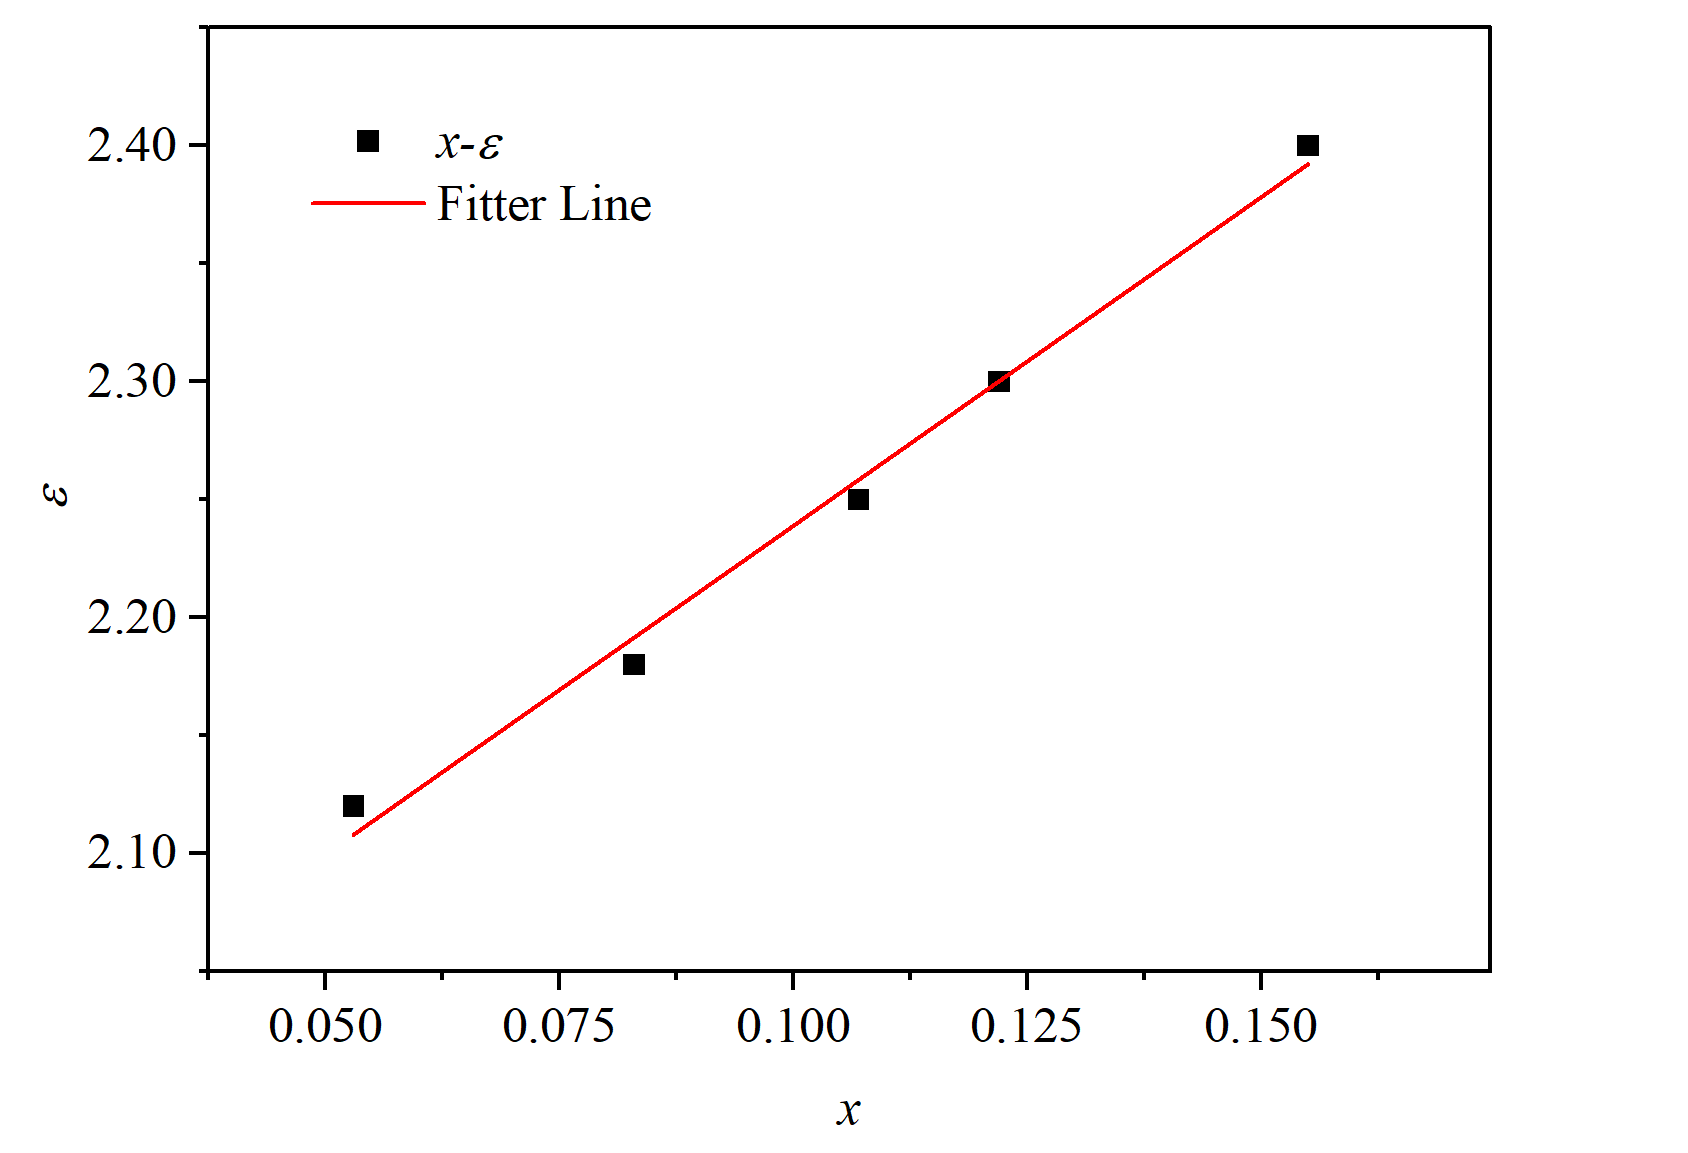
\includegraphics[width=.8\textwidth]{figures/1-1.png}
    \bicaption{最大气泡压力法:正丁醇水溶液 $\gamma-\ln c$ 等温曲线及拟合直线}{Maximum Bubble Pressure Method: $\gamma-\ln c$ isotherm and fitted curve}
    \label{fig:1}
\end{figure}

\begin{table}[htbp]
    \centering
    \bicaption{$\gamma-\ln c$ 曲线线性区取点相关数据}{Point data in the linear area of the $\gamma-\ln c$ curve}
    \begin{tabular}{cccc}
    \toprule
    $c / \mathrm{mol} \cdot \mathrm{L}^{-1}$ & $\ln \left(c / \mathrm{mol} \cdot \mathrm{L}^{-1}\right)$ & $\gamma / \mathrm{mN} \cdot \mathrm{m}^{-1}$ & $\sigma_\gamma$ \\
    \midrule
    0.150 & -1.897 & 47.96 & 0.48 \\
    0.200 & -1.609 & 44.51 & 0.48 \\
    0.300 & -1.204 & 38.65 & 0.45 \\
    0.400 & -0.916 & 35.45 & 0.44 \\
    0.450 & -0.799 & 33.94 & 0.43 \\
    \bottomrule
    \end{tabular}
    \label{tab:4}
\end{table}

根据公式 \eqref{eq:2},有
$$
\Gamma_{\infty}=-\frac{1}{R T} \cdot \frac{\mathrm{d} \gamma}{\mathrm{d} \ln c}=-\frac{-12.87 \times 10^{-3}}{8.314 \times 303.15} \mathrm{~mol} \cdot \mathrm{m}^{-2}=5.11 \times 10^{-6} \mathrm{~mol} \cdot \mathrm{m}^{-2}
$$

已知 $\sigma_{\frac{\mathrm{d} \gamma}{\mathrm{dln} c}}=0.31, \sigma_T=0.01$,则由误差传递公式,有:
$$
\begin{aligned}
\sigma_{\Gamma_{\infty}} & =\sqrt{\left(\frac{1}{R T} \cdot \frac{\sigma_T}{T}\right)^2+\left(\frac{1}{R T} \cdot \sigma_{\frac{\mathrm{d} \gamma}{\mathrm{dln} c}}\right)^2} \\
& =\frac{1}{8.314 \times 303.15} \sqrt{\left(\frac{0.01}{303.15}\right)^2+\left(0.31 \times 10^{-3}\right)^2} \\
& =0.12 \times 10^{-6} \mathrm{~mol} \cdot \mathrm{m}^{-2}
\end{aligned}
$$

最终可得,最大气泡法测得的饱和吸附量:
$$
\Gamma_{\infty}=(5.11 \pm 0.12) \times 10^{-6} \mathrm{~mol} \cdot \mathrm{m}^{-2}
$$

分子吸附面积:
$$
q = \frac{1}{N_{\mathrm{A}}\Gamma_{\infty}} = \frac{1}{5.11 \times 10^{-6} \times 6.022 \times 10^{23}} \times 10^{18} \mathrm{~nm}^2=0.325 \mathrm{~nm}^2
$$

其误差:
$$
\sigma_q=\sqrt{\left(\frac{\sigma_{\Gamma_{\infty}}}{\Gamma_{\infty}^2 N_A}\right)^2}=\sqrt{\left(\frac{0.12 \times 10^{-6}}{\left(5.11 \times 10^{-6}\right)^2 \times 6.022 \times 10^{23}} \times 10^{18}\right)^2}=0.0076 \mathrm{~nm}^2
$$

最终可得,最大气泡法测得的分子吸附面积:
$$
q = (0.325\pm 0.008) \mathrm{~nm}^2
$$

\subsubsection{吊片法}

由于吊片法测定表面张力时,读数波动过大,本人根据实际读数波动的范围估计其误差$\sigma_\gamma = \SI{1}{mN\cdot m^{-1}}$。与 3.2.1 类似,进行带$y$误差的线性回归,使用matplotlab作图,选择用于线性拟合的点如表 \ref{tab:5},得到图 \ref{fig:2},回归直线的表达式为:

\begin{equation*}
    \frac{\gamma}{\si{mN\cdot m^{-1}}} = (-13.70 \pm 0.62)\ln\left(\frac{ c_{n\ce{BuOH}}}{\si{mol\cdot L^{-1}}}\right) + (26.86 \pm 0.83);\quad R^2 = 0.9940
\end{equation*}

\begin{figure}[htbp]
    \centering
    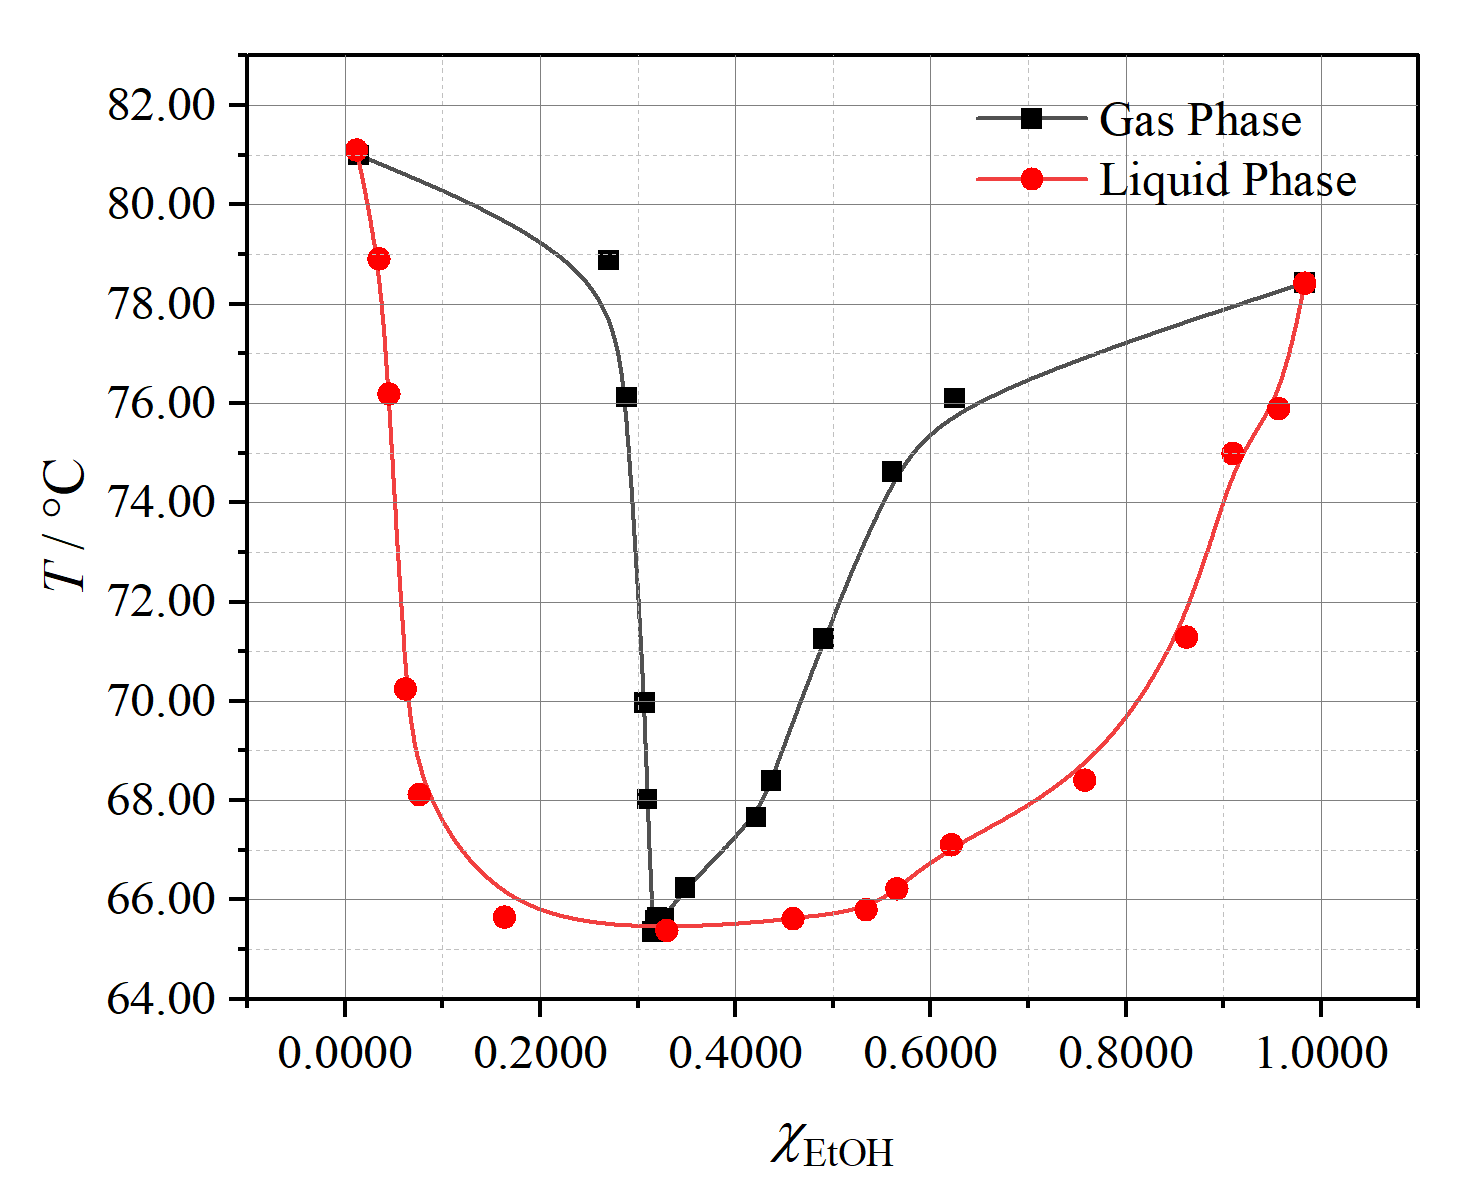
\includegraphics[width=.8\textwidth]{figures/1-2.png}
    \bicaption{吊片法:正丁醇水溶液 $\gamma-\ln c$ 等温曲线及拟合直线}{Wilhelmy Plate Method: $\gamma-\ln c$ isotherm and fitted curve}
    \label{fig:2}
\end{figure}

\begin{table}[htbp]
    \centering
    \bicaption{$\gamma-\ln c$ 曲线线性区取点相关数据}{Point data in the linear area of the $\gamma-\ln c$ curve}
    \begin{tabular}{cccc}
    \toprule
    $c / \mathrm{mol} \cdot \mathrm{L}^{-1}$ & $\ln \left(c / \mathrm{mol} \cdot \mathrm{L}^{-1}\right)$ & $\gamma / \mathrm{mN} \cdot \mathrm{m}^{-1}$ & $\sigma_\gamma$ \\
    \midrule
    0.150 & -1.897 & 52.24 & 1 \\
    0.200 & -1.609 & 49.56 & 1 \\
    0.300 & -1.204 & 43.66 & 1 \\
    0.400 & -0.916 & 39.28 & 1 \\
    0.450 & -0.799 & 37.53 & 1 \\
    \bottomrule
    \end{tabular}
    \label{tab:5}
\end{table}

根据公式 \eqref{eq:2},有
$$
\Gamma_{\infty}=-\frac{1}{R T} \cdot \frac{\mathrm{d} \gamma}{\mathrm{d} \ln c}=-\frac{-13.70 \times 10^{-3}}{8.314 \times 303.15} \mathrm{~mol} \cdot \mathrm{m}^{-2}=5.44 \times 10^{-6} \mathrm{~mol} \cdot \mathrm{m}^{-2}
$$

已知 $\sigma_{\frac{\mathrm{d} \gamma}{\mathrm{dln} c}}=0.62, \sigma_T=0.01$,则由误差传递公式,有:
$$
\begin{aligned}
\sigma_{\Gamma_{\infty}} & =\sqrt{\left(\frac{1}{R T} \cdot \frac{\sigma_T}{T}\right)^2+\left(\frac{1}{R T} \cdot \sigma_{\frac{\mathrm{d} \gamma}{\mathrm{dln} c}}\right)^2} \\
& =\frac{1}{8.314 \times 303.15} \sqrt{\left(\frac{0.01}{303.15}\right)^2+\left(0.62 \times 10^{-3}\right)^2} \\
& =0.24 \times 10^{-6} \mathrm{~mol} \cdot \mathrm{m}^{-2}
\end{aligned}
$$

最终可得,吊片法测得的饱和吸附量:
$$
\Gamma_{\infty}=(5.44 \pm 0.24) \times 10^{-6} \mathrm{~mol} \cdot \mathrm{m}^{-2}
$$

分子吸附面积:
$$
q = \frac{1}{N_{\mathrm{A}}\Gamma_{\infty}} = \frac{1}{5.44 \times 10^{-6} \times 6.022 \times 10^{23}} \times 10^{18} \mathrm{~nm}^2=0.305 \mathrm{~nm}^2
$$

其误差:
$$
\sigma_q=\sqrt{\left(\frac{\sigma_{\Gamma_{\infty}}}{\Gamma_{\infty}^2 N_A}\right)^2}=\sqrt{\left(\frac{0.24 \times 10^{-6}}{\left(5.44 \times 10^{-6}\right)^2 \times 6.022 \times 10^{23}} \times 10^{18}\right)^2}=0.013 \mathrm{~nm}^2
$$

最终可得,吊片法测得的分子吸附面积:
$$
q = (0.305\pm 0.013) \mathrm{~nm}^2
$$

\subsection{饱和吸附时实际分子面积的计算}

因为 $\Gamma$ 实际上是一个过剩量,即使其等于 0(无吸附),表面上仍有溶质分子。故计算 $q$ 时忽略了表面上原有的溶质分子。对于较浓的溶液,在计算表面上溶质分子数时,除了吸附分子还应考虑原有分子。若 $\Gamma$ 以 $\mathrm{mol/m}^2$ 为单位,$c$ 以 $\mathrm{mol/dm}^3$ 为单位,$q_c$ 以 $\mathrm{nm}^2$ 为单位,则实际溶液浓度为 $c$ 时的吸附量为:
$$
q_c = \frac{10^{18}}{\Gamma N_A + 100 \times \left( c N_A \right)^{2/3}}
$$

考虑在高浓度时,饱和吸附时的实际分子面积:
\begin{equation}\label{eq:6}
    q_c = \frac{10^{18}}{\Gamma_\infty N_A + 100 \times \left( c N_A \right)^{2/3}}
\end{equation}


其误差可以表示为:
\begin{equation}\label{eq:7}
    \sigma_{q_c}=\sqrt{\left(\frac{N_A \cdot \sigma_{\Gamma_{\infty}}}{\left(\Gamma_{\infty} N_A+\left(c N_A\right)^{2 / 3}\right)^2}\right)^2+\left(\frac{2}{3} \cdot \frac{c^{-1 / 3} N_A^{2 / 3} \cdot \sigma_c}{\left(\Gamma_{\infty} N_A+\left(c N_A\right)^{2 / 3}\right)^2}\right)^2}
\end{equation}


根据公式 \eqref{eq:6}、\eqref{eq:7},可以计算在饱和吸附时,不同浓度的正丁醇溶液的实际分子面积及其不确定度,两种方法的计算结果分别如表 \ref{tab:6}。

\begin{table}[ht]
\centering
\bicaption{不同浓度下的$q_c$值}{Maximum Bubble Pressure Method: $q_c$ values at Different Concentrations}
\begin{tabular}{ccccc}
\toprule
\multirow{2}{*}{$c / \mathrm{mol \cdot L^{-1}}$} & \multicolumn{2}{c}{最大气泡压力法} & \multicolumn{2}{c}{吊片法} \\
& $\Gamma_\infty/\si{mol\cdot m^{-2}}$ & $q_c / \mathrm{nm^2}$ & $\Gamma_\infty/\si{mol\cdot m^{-2}}$ & $q_c / \mathrm{nm^2}$ \\
\midrule
0.220 & \multirow{5}{*}{0.511} & 0.300 $\pm$ 0.008 & \multirow{5}{*}{0.544} & 0.283 $\pm$ 0.013\\
0.329 & & 0.293 $\pm$ 0.008 & & 0.277 $\pm$ 0.013\\
0.439 & & 0.287 $\pm$ 0.008 & & 0.271 $\pm$ 0.013\\
0.550 & & 0.281 $\pm$ 0.008 & & 0.266 $\pm$ 0.013\\
0.740 & & 0.273 $\pm$ 0.008 & & 0.259 $\pm$ 0.013\\
\bottomrule
\end{tabular}
\label{tab:6}
\end{table}












\section{结果与讨论}

\subsection{探索实验:动态法测定 \ce{H2O} 沸点时的读数问题与实验改进}

由于在动态法测定 \ce{H2O} 沸点时,温度-气压计的温度示数难以稳定,会不断跳动增加;为了找出最佳的读数时机与方式,我进行了一系列探索实验:
\begin{enumerate}
    \item 在温度缓慢上升平台期的起始与终点分别取点,进行线性拟合,尝试通过物理量的计算结果准确度来比较不同读数方式的优劣。但遗憾的是,由于动态法存在较大的读数误差,这样的误差传递到拟合直线中,造成了参数 $a$ 不确定度显著大于静态法的参数。而参数 $a$ 又与有明确文献值的摩尔汽化焓 $\Delta_1^{g} H_{m}$ 直接相关。$\Delta_1^{g} H_{1,m}, \Delta_1^{g} H_{2,m},\Delta_1^{g} H_{m}$ 均有过大的误差,导致彼此之间没有显著性差别,无法通过实验结果的准确度来衡量读数方式的优劣,也无法做出最终的判断。
    \item 最终体系连通环境后,测定水在环境气压下的沸点时读数时间的选取。这一部分也面临着同样的不确定度过大的问题,无法得出明确结论。
\end{enumerate}

虽然两项探索实验均没有通过不同读数方式准确性的比较,得出最终孰优孰劣的结论,但是通过进行探索实验,积累了一定的实验经验,基于这些经验,可以提出如下两方面可能的动态法实验改进方法:
\begin{enumerate}
    \item \textbf{控温方式的改进}:在原本的实验\cite{pcl2002}中,并没有明确说明在一定气压下 \ce{H2O} 沸腾的平台期如何控温,为此,我建议:在一定气压下 \ce{H2O} 将要沸腾时,将加热套的加热功率逐渐缓缓调低,以免剧烈沸腾;如果 \ce{H2O} 沸腾较为剧烈,可以继续尽可能降低加热套功率,直至能保持水温和沸腾的最低功率,此时,理想情况下水温可以保持恒定。
    \begin{itemize}
        \item 需要注意的是,由于体系温度逐渐升高,其与环境的热交换功率也在提高,加热套的最低加热功率需要相应的提高。
    \end{itemize}
    \item \textbf{读数方式的改进}:在原本的实验\cite{pcl2002}中,只读取1组数据;而通过我提出的控温方式,可以实现在当 \ce{H2O} 温度稳定时,读取3次温度-气压取平均,即为该气压下水的沸点,以显著降低结果的误差,且有望使得动态法实现类似于静态法的精度。
\end{enumerate}

\subsection{结论}

本实验使用静态法测量 \ce{CCl4} 在不同温度下的饱和蒸气压,测得 \ce{CCl4} 的常压沸点为 \( T_b = 348.97 \pm 0.02\,\mathrm{K} \);根据实验数据作出 \( p-T \) 曲线和 \( \ln \left( \dfrac{p}{p^\ominus} \right) \) 拟合直线,根据拟合直线计算 \ce{CCl4} 的标准大气压下的沸点为 \( T_b = 349.3 \pm 1.2\,\mathrm{K} \),平均摩尔气化热为 \( \Delta_1^{g} H_m = 32.28 \pm 0.08\,\mathrm{kJ\cdot mol^{-1}} \),摩尔气化熵为 \( \Delta_1^{g} S_m = 92.53 \pm 0.23\,\mathrm{J\cdot K^{-1}\cdot mol^{-1}} \)。各热力学数据计算值与文献参考值较为接近。

使用动态法测量 \ce{H2O} 在不同温度下的饱和蒸气压,测得 \ce{H2O} 的在当前大气压 \( 99.84\,\mathrm{kPa} \) 下的沸点为 \( T_b = 373.53 \pm 0.03\,\mathrm{K} \);根据实验数据作出 \( p-T \) 曲线和 \( \ln \left( \dfrac{p}{p^\ominus} \right) \) 拟合直线,根据拟合直线计算 \ce{H2O} 的标准大气压下的沸点为 \( T_b = 373 \pm 3\,\mathrm{K} \),平均摩尔气化热为 \( \Delta_1^{g} H_m = 41.01 \pm 0.08\,\mathrm{kJ\cdot mol^{-1}} \),摩尔气化熵为 \( \Delta_1^{g} S_m = 109.8 \pm 0.2\,\mathrm{J\cdot K^{-1}\cdot mol^{-1}} \)。各热力学数据计算值与文献参考值较为接近。


本实验验证了 \ce{CCl4} 的摩尔气化熵大致符合褚鲁统规则的预测,而 \ce{H2O} 不符合褚鲁统规则,分析可能原因是 \ce{H2O} 中分子间氢键的存在使得摩尔气化熵偏离褚鲁统规则。并探索了动态法测定 \ce{H2O} 沸点时不同读数方式所得到的结果的差别,从控温、读数两方面提出了改进动态法测沸点实验,提升准确度与精密性的改进方法。



% 参考文献
\nocite{*}
\bibliographystyle{achemso}
\bibliography{reference}

\end{document}